\chapter{Experimentación}\label{ch:Experimentación}

Esta sección tiene como objetivo mostrar el correcto funcionamiento las funciones documentadas en la sección \ref{ch:Impl}. Para ello las aplicaremos sobre conjuntos de datos correspondientes a casos de aplicación reales, así como a conjuntos artificiales.

Cabe destacar que los parámetros dados como argumento a las funciones son los especificados por defecto en la sección \ref{ch:Impl} a no ser que se especifique lo contrario, es decir, no se han optimizado para los datos concretos a los que se aplican en cada ocasión. La optimización de parámetros queda a cargo del usuario, que deberá realizar un estudio sobre los mismos para adaptarlos al problema concreto que intenta resolver.

\section{Conjuntos de datos considerados}

Tal y como ya se ha mencionado, tomaremos conjuntos de datos reales y artificiales para poner a prueba los 5 métodos implementados. Teniendo en cuenta dicha distinción, a continuación se detallan los pormenores de cada uno de ellos.

\subsection{Conjuntos de datos reales}

Consideraremos 4 conjuntos de datos correspondientes a casos reales de aplicación de técnicas de \acf{AA}:

\begin{itemize}
	
	\item \textbf{Conjunto de datos \textit{Iris}}: el conjunto de datos Iris (\textit{Iris dataset}) es uno de los más empleados en \acs{AA}. Famoso por ser objeto del primer intento de aplicación de métodos de clustering por el biólogo Ronald Fisher en 1936, quien intentaba obtener un método para clasificar flores de la especie Iris en sus tres subespecies: \textit{iris setosa}, \textit{iris virginica} e \textit{iris versicolor}. Compuesto por un total de 150 muestras de 3 clases distintas, caracterizadas cada una por 4 atributos en el dominio de los números reales positivos, a saber: altura del sépalo, anchura del sépalo, altura del pétalo y anchura del pétalo. Aunque solo consideraremos las dos primeras, por comodidad para la representación. La Figura \ref{fig:figure21} muestra las distribución de las dos primeras variables del conjunto de datos Iris.
	
	\item \textbf{Conjunto de datos \textit{Wine}}: el conjunto de datos Wine (\textit{Wine dataset}) recoge 178 muestras de 3 clases de vinos distintas, caracterizadas cada una por 13 atributos en el dominio de los números reales positivos. Algunos de estos atributos son: contenido de alcohol, contenido de ácido málico, contenido de magnesio, etc.
	
	\item \textbf{Conjunto de datos \textit{Breast Cancer}}: el conjunto de datos Breast Cancer (\textit{Breast Cancer dataset}) recoge 569 asociadas cada una a una paciente que padecía o no de cáncer de mama (2 clases), cada muestra viene caracterizada por 30 atributos en el dominio de los números reales positivos. Algunos de los atributos son: edad de la paciente, tamaño del tumor, mama afectada, etc.
	
	\item \textbf{Conjunto de datos \textit{Glass}}: el conjunto de datos Glass (\textit{Glass dataset}) recoge 214 muestras de 6 clases de cristal distintas, caracterizadas cada una por 10 atributos en multitud de dominios. Algunos de estos atributos son: indice reactivo, contenido en magnesio, contenido en aluminio, finalidad de uso, etc.
	
\end{itemize}


\begin{figure}[!h]
	\centering
	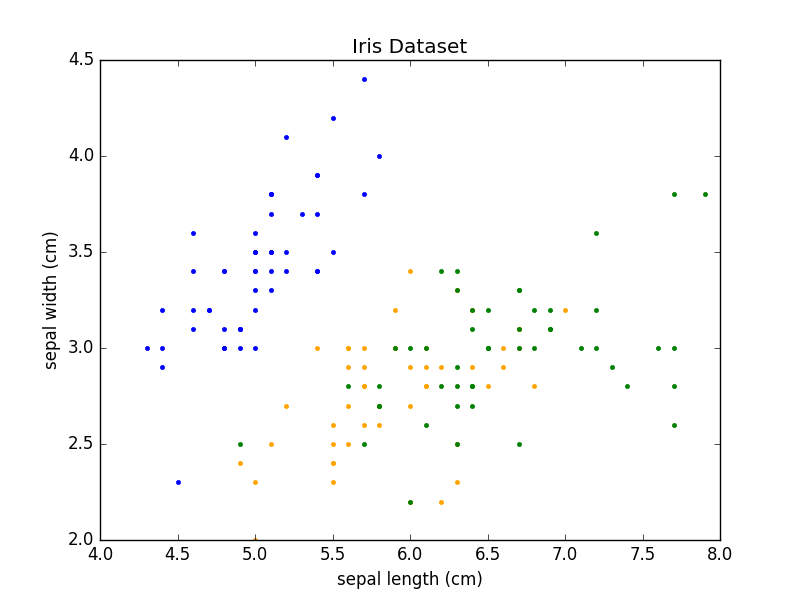
\includegraphics[scale=0.5]{imagenes/c6/IrisSet}
	\caption[Conjunto de datos Iris]{Conjunto de datos Iris.}\label{fig:figure21}
\end{figure}

\subsection{Conjuntos de datos artificiales}

En el caso de los conjuntos de datos artificiales el objetivo es generar clusters con una geometría concreta, para ello solo son necesarios dos atributos ($x$ e $y$) y un número de muestras arbitrario, que en este caso estableceremos como 300.

La Figura \ref{fig:figure22} muestran los 4 conjuntos de datos generados de manera artificial. Por simplicidad nos referiremos a cada uno de ellos por su identificador en ingles, que aparece en la anotación bajo cada imagen.

\begin{figure}[bth]
	\myfloatalign
	\subfloat[\textit{Rand Dataset}]
	{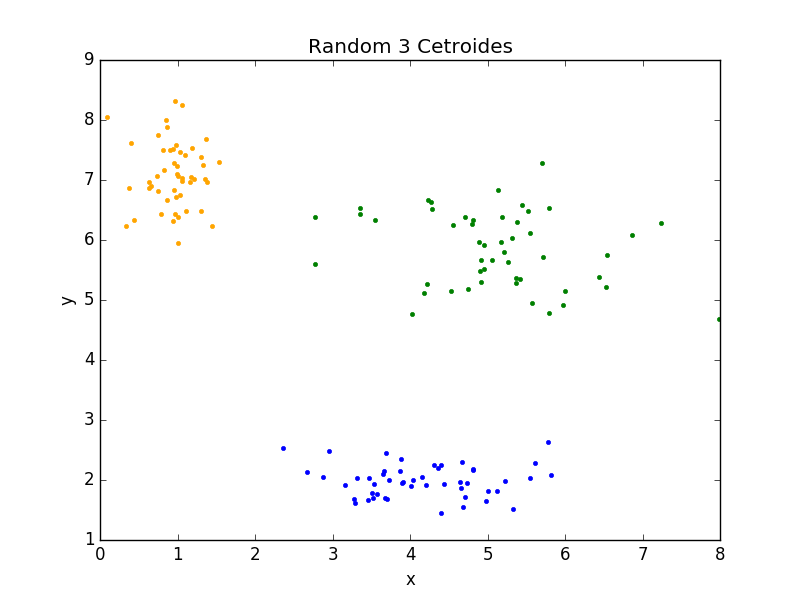
\includegraphics[width=.4\linewidth]{imagenes/c6/ArtifSets/RandSet}}
	\subfloat[\textit{Spirals Dataset}]
	{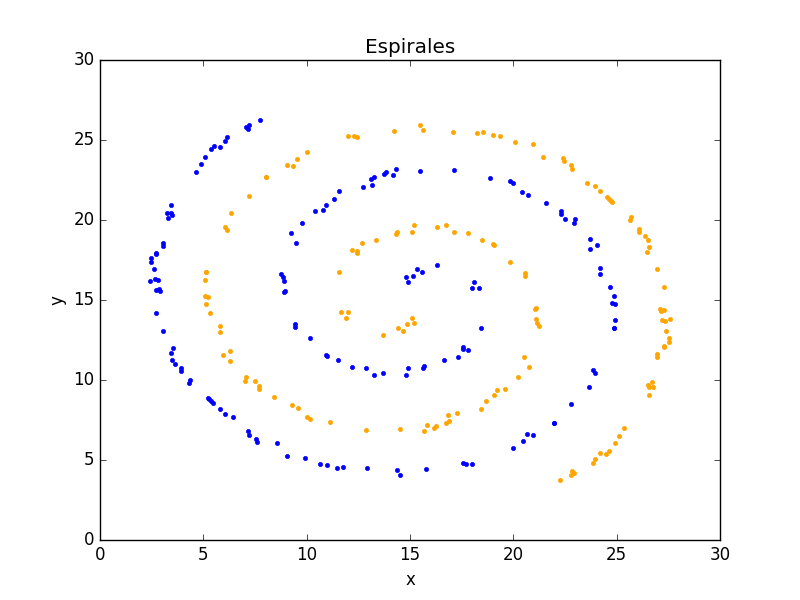
\includegraphics[width=.4\linewidth]{imagenes/c6/ArtifSets/SpiralSet}}\\
	\subfloat[\textit{Circles Dataset}]
	{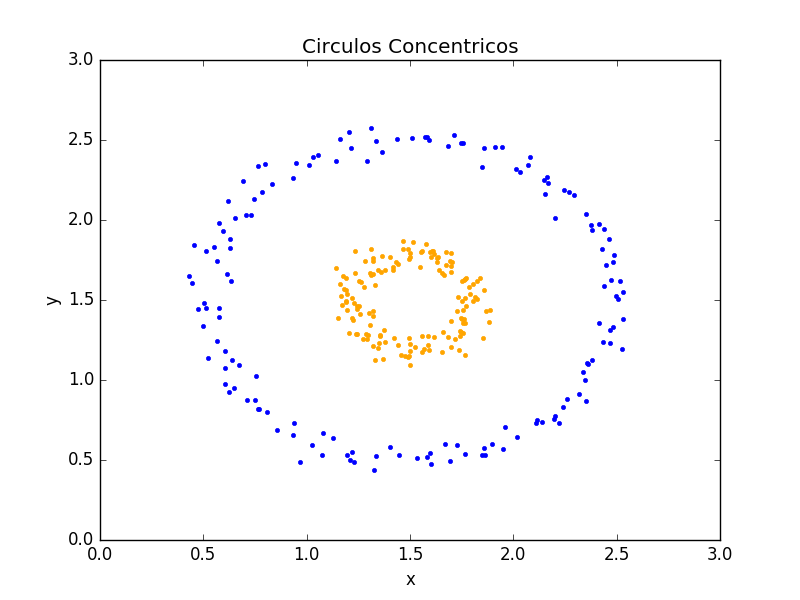
\includegraphics[width=.4\linewidth]{imagenes/c6/ArtifSets/Circles}}
	\subfloat[\textit{Moons Dataset}]
	{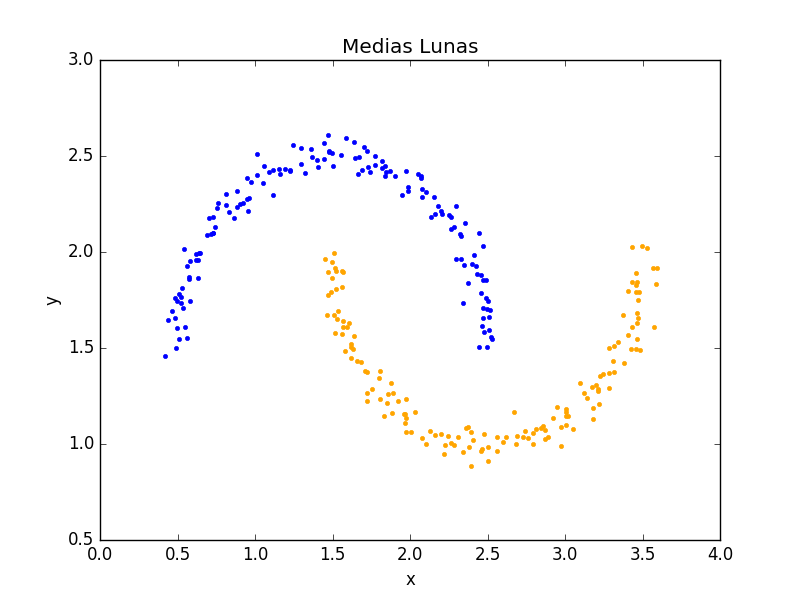
\includegraphics[width=.4\linewidth]{imagenes/c6/ArtifSets/MoonsSet}}
	\caption{Conjuntos de datos artificiales.}\label{fig:figure22}
\end{figure}

\section{Medida del error}






